\documentclass{article}

\author{Pedro Henrique Limeira da Cruz}
\title{EM461 - Mecânica dos Fluidos I}

\usepackage[margin=0.8in]{geometry}
\usepackage{indentfirst}
\usepackage{fancyhdr}
\usepackage{tcolorbox}
\usepackage{graphicx}
\usepackage{amsmath}
\usepackage{amssymb}
\usepackage{tabularx}
\usepackage{subcaption}
\usepackage{float}
\usepackage{array}
\usepackage{wrapfig}

% Create a new command to be used in the align environment in multiple line equations do only the last equation is numbered  
\newcommand{\n}{\nonumber \\ }
\makeatletter
\let\inserttitle\@title
\makeatother
% Set the style of the page 
\pagestyle{fancy}
\fancyhf{}
\rhead{Pedro Henrique L. da Cruz}
\lhead{\inserttitle}
\rfoot{Page \thepage}

\usepackage{hyperref}
\hypersetup{
    colorlinks=true,
    linkcolor=black,
    filecolor=magenta,
    urlcolor=cyan,
}

\renewcommand\tabularxcolumn[1]{m{#1}}%


% Begin the Document 
\begin{document}

\maketitle
\thispagestyle{empty}

% Add the image inside a figure in as the first page
% \begin{figure}[h]
%     \begin{center}
%         
\includegraphics[scale = 0.15]{/Users/pedrocruz/Documents/UNICAMP/ES101/ES101 - Robotic Arm/img/unicamp.png}
%     \end{center}
% \end{figure}

% Change to the Next page 
\newpage
\tableofcontents
\newpage

\section{Estática dos Fluidos}
Antes de começarmos nossos estudos sobre a mecânica dos fluidos em movimento, iremos revisar (ou para alguns introduzir) a estática de fluidos.

\subsection{Equação Base - Estática de Fluidos}
A equação mais básica da estática de fluidos é aquela que modela o campo de pressão em um fluido estático. A partir das experiências do dia-a-dia podemos verificar o principal aspecto
sobre a pressão em uma coluna de fluido estático:

\begin{center}
    \textbf{A pressão Aumenta com a Profundidade}
\end{center}

A partir disso, e com a intenção de modelarmos matematicamente o sistema, fazemos a análise mais básica de mecânica estática, a lei de Newton. Para esse caso, entretanto, como estamos
falando de um fluido e não de um corpo concentrado, iremos aplicar a lei de newton em um cenário diferencial, para lidarmos com pequenas massas (ou pequenos volumes) do fluido, como mostra a equação \ref{eq:newton_diff_base}:
\begin{align}
    d\vec{F}_{resultante}= \vec a dm \label{eq:newton_diff_base}
\end{align}

A partir disso, como temos nossa lei de newton básica (mas agora aplicada para o problemas diferencial de fluidos), podemos prosseguir e identificar as forças envolvidas.

A primeira força de campo que iremos ver e que atua nos problemas de estática de fluidos é a força oriunda da \emph{gravidade}, quando analisamos um pequeno volume diferencial do fluido, dada por:
\begin{align}
    d\vec{F}_B = \vec{g}\rho d \forall \label{eq:forca_peso}
\end{align}

Onde:
\begin{itemize}
    \item $\rho$: Massa específica. Para problemas que estaremos analisando é constante em função tanto do tempo quanto posição.
    \item $\forall$: Volume do elemento, dada em coordenadas cartesianas tal que $d\forall = dx \ dy \ dz$
    \item $g$: Aceleração da gravidade.
\end{itemize}

A segunda força que iremos analisar agora é a \textbf{única força de superfície} presente, tendo em vista que estamos abordado a estática de fluidos e, por conseguinte, não há a presença
de tensão de cisalhamento, é a \textbf{força de pressão de superfície} $p = p(x, y, z)$ (um vetor com três componentes), que varia conforme a posição dentro do fluido. Podemos entender essa pressão de superfície como sendo a
\textbf{Pressão exercida pela coluna de fluido ao redor do volume diferencial sendo estudado}.

A partir disso, temos a Lei de Newton que governa o problema diferencial do fluido (dado pela equação \ref{eq:newton_diff_base}) e temos que as únicas forças que atua no nosso problema são a
força de pressão $p(x, y, z)$ e a força peso do volume diferencial sob análise. Como estamos lidando com um problema de estática a somatória de todas as forças precisa ser zero, temos:

\begin{align}
    d\vec{F} = (-\nabla p + \rho \vec{g}) d\forall \Rightarrow \frac{d\vec{F}}{d\forall} = -\nabla p + \rho \vec g \label{eq:newton_estatica_de_fluidos}
\end{align}

Onde temos então a equação final \ref{eq:newton_estatica_de_fluidos}, que representa a força resultante por unidade de volume, que ao igualarmos a zero resulta em:

\begin{align}
    -\nabla p & + \rho \vec g = 0\label{eq:newton_resultante_estatica_de_fluidos}
\end{align}

Onde:
\begin{itemize}
    \item $-\nabla p$: Força de pressão resultante por unidade de volume em um ponto. Representado pelo vetor gradiente com uma componente $x$ uma $y$ e uma $z$
    \item $\rho \vec g$: Força de campo (gravitacional) por unidade de volume em um ponto
\end{itemize}

\subsection{Variação de Pressão em um Fluido Estático}
A seção anterior foi de suma importância por introduzir a modelagem amtemática básica para a estática de fluidos, com a equação \ref{eq:newton_resultante_estatica_de_fluidos}. A partir
disso, podemos dissecar tal equação e relacionarmos o que sabemos na prática (que a pressão aumenta com a profundidade) com a modelagem.

Para tal, precisamos primeiro considerar que estamos lidando com um \textbf{líquido incompressível}, de tal forma que $\rho=const$ e também que a gravidade é uma constante e aponta na
direção $z$ somente. A partir disso, precisamos analisar a equação \ref{eq:newton_resultante_estatica_de_fluidos} somente no eixo $z$ , resultando em:

\begin{align}
    -\nabla p + \rho \vec g                      & = 0 \n
    -\frac{\partial p}{\partial z} + \rho (-g_z) & = 0 \n
    -\frac{dp}{d z} + \rho (-g_z)                & = 0 \label{eq:diff_inicial_pressao}                      \\
    dp                                           & = +\rho g_z dz \n
    \int^p_{p_0} dp                              & = \int^z_{z_0} \rho g_z dz \n
    p - p_0                                      & = \rho g_z (z- z_0) \n
    \Delta p                                     & = \rho g h  \label{eq:final_delta_p_estatica_de_fluidos}
\end{align}

É importante ressaltar que, a equação \ref{eq:final_delta_p_estatica_de_fluidos} só é valida para:
\begin{itemize}
    \item Fluido Estático
    \item A gravidade é a única força de campo
    \item O eixo $z$ é vertical voltado para cima
\end{itemize}

Além disso, a equação \ref{eq:diff_inicial_pressao} é importante para os casos em que o fluido não é incompressível (e por conseguinte a massa específica $\rho$ pode variar com a pressão
$p$). Para esses casos, devemos partir nossas contas dessa equação e fazer a integral para o devido $\rho = f(p)$, como é nos casos dos gases ideais. Importante ressaltar que o sinal da
gravidade é negativo pois o eixo $z$ é positivo para cima, \textbf{se o eixo $z$ for positivo para baixo o sinal da gravidade na equação \ref{eq:diff_inicial_pressao} seria positivo}.


\newpage

\subsection{Variação de Pressão Em um Gás Ideal}
Como dito na parte anterior, há casos que lidaremos com fluidos compressíveis, sendo o mais notório deles os chamados \textbf{gases ideais}, onde:
\begin{align}
    p & = \rho RT \therefore \rho = \frac{P}{RT} \label{eq:gases_ideais}
\end{align}

Onde:
\begin{itemize}
    \item $T$: Temperatura em Kelvin
    \item $P$: Pressão
    \item $\rho$: Massa Específica
    \item $R$: Constante universal dos gases (tabelada)
\end{itemize}

A partir da equação \ref{eq:gases_ideais}, e da equação \ref{eq:diff_inicial_pressao}, somos capazes de determinar uma expressão para a pressão em um gás ideal:
\begin{align}
    dp                         & = - \rho g dz \n
    dp                         & = - \frac{p}{RT} g dz \n
    \frac{1}{p} dp             & = -\frac{1}{RT} g dz \n
    \int^p_{p_0}\frac{1}{p} dp & = -\int^z_{z_0}\frac{1}{RT} g dz \n
    \ln{(p/p_0)}               & = -\frac{g}{RT} (z - z_0)
\end{align}

\newpage

\subsection{One Pager - Estática de Fluidos}

\begin{table}[h]\tiny
    \begin{tabularx}{\textwidth}{|l|c|X|}\hline
        \textbf{Uso}                                         & \textbf{Equação}                                  & \textbf{Descrição}                                                                                                                               \\ \hline

        \rule{0pt}{7ex}Estática de Fluidos - Geral           & $d\vec{F} = \vec{a} dm$                           & A segunda Lei de Newton em um formato infinitesimal, base para a análise de forças em Estática dos Fluidos.                                      \\[4ex] \hline
        \rule{0pt}{7ex}Estática de Fluidos - Geral           & $- \nabla p + \rho \vec g = 0$                    & A aplicação da segunda lei para um volume infinitesimal de um fluido estático apensa sob pressão e gravidade. OBS: $\nabla p$ representa o vetor
        gradiente nas três direções da pressão.                                                                                                                                                                                                                     \\ [4ex]\hline

        \rule{0pt}{7ex}Variação de Pressão - Fluido Estático & $dp/dz = -\rho g_z \Rightarrow dp = -\rho g_z dz$ & Aplicação específica da fórmula do volume apensa sob pressão, e gravidade somente no eixo
        $y$, base para problemas para calcular variação de pressão a depender de $z$ (especialmente se $\rho$ depender de $z$ ou de $p$ como no exemplo de gases ideais)                                                                                            \\ [4ex]\hline

        \rule{0pt}{7ex}Variação de Pressão - Fluido Estático & $\Delta p = \rho g h$                             & Variação de pressão para fluidos incompressíveis, estáticos.                                                                                     \\ [4ex]\hline

        \rule{0pt}{7ex}Variação de Pressão - Gás Ideal       & $p = \rho RT \Rightarrow \rho = p/RT$             & Fórmula que relaciona pressão e massa específica $\rho$ dos gases ideais.                                                                        \\ [4ex]\hline

        \rule{0pt}{7ex}Variação de Pressão - Gás Ideal       & $\ln{(p/p_0)} = -(g/RT)(z - z_0)$                 & Fórmula para variação da pressão em gasses ideais, oriundo da integração da equação diferencial geral de variação
        pressão, em conjunto com a equação que expressa $\rho$ em função de $p$ para gases ideais acima.                                                                                                                                                            \\ [4ex]\hline
    \end{tabularx}
\end{table}
\newpage

\section{Conceitos Fundamentais Dinâmica dos Fluidos}
Agora que revemos os conceitos mais básicos de Estática dos Fluidos, iremos então explorar os principais conceitos de Dinâmica dos Fluidos, sendo o primeiro deles a ideia de
campo de velocidade.

\subsection{Campo de Velocidade}
Algo muito importante de internalizarmos entes de falarmos sobre a velocidade de um líquido é que ele não é uma partícula, mas sim um conjunto "contínuo" de partículas, por isso chamamos
um fluido de um "contínuo". Como resultado direto disso, temos que a velocidade de um certo volume de fluido pode depender não somente do tempo (como estamos mais acostumados com corpos
rígidos), mas também pode depender da posição que está sendo analisada dentro de tal fluido, \emph{i.e} a velocidade é um função da posição da partícula de análise como também do tempo:
\begin{align}
    \vec V = \vec V (x, y, z, t) = u \hat i + v \hat j + w \hat k \label{eq:campo_velocidade}
\end{align}

A partir disso, podemos agrupar os diferentes tipo de escoamento de fluidos em relação a:
\begin{itemize}
    \item \textbf{Dimensões de Escoamento}:
          \subitem $\hookrightarrow$ \underline{Escoamento Uni-Dimensional}: O campo de velocidade, no que tange posição, muda em relação a somente uma coordenada.
          \subitem $\hookrightarrow$ \underline{Escoamento Bi-Dimensional}: O campo de velocidade, no que tange posição, muda em relação a  duas coordenadas.
          \subitem $\hookrightarrow$ \underline{Escoamento Tri-Dimensional}: O campo de velocidade, no que tange posição, muda em relação a três coordenadas.
    \item \textbf{Variação no Tempo}:
          \subitem $\hookrightarrow$\underline{Regime Permanente}: A velocidade nem a massa específica variam com o tempo.
          \subitem $\hookrightarrow$\underline{Regime Transiente}: As propriedades do fluido podem variar em relação ao tempo.
\end{itemize}

\subsection{Linhas de Caracterização}
Para estudarmos o comportamento de um fluido, principalmente da sua interação com outros corpos e superfícies, nós usamos diferentes técnicas, chamadas de linhas de caracterização, sendo
elas:
\begin{itemize}
    \item \textbf{Linhas de Tempo}: Análise de Várias partículas adjacentes, em um determinado instante. Obtida via experimento.
    \item \textbf{Linhas de Trajetória}: Análise do caminho traçado por uma partícula em movimento. Obtida via experimento.
    \item \textbf{Linhas de Emissão}: Linha que traça todos os caminhos que particulas que passaram por um determinado ponto no espaço. Obtida via experimento.
    \item \textbf{Linhas de Corrente}: Linhas tangente à direção e velocidade de escoamento em cada ponto do campo. Obtida Matematicamente.
\end{itemize}

Sendo que é importante ressaltar que para regime permanente, todas coincidem.

A que mais vamos ver, por ser obtida matematicamente, é a linha de corrente, que é dada por:
\begin{align}
    \frac{dy}{dx} \big{)}_{linha \ de \ corrente} = \frac{v}{u}, \ \ \begin{cases}
                                                                         v = v_y \\
                                                                         u = v_x
                                                                     \end{cases}
\end{align}

A partir disso somos capazes de isolar $dx$ com tudo que depende de $x$, e $dy$ com tudo que depende de $y$ e integrar para acharmos uma equação que depende de $x,y$ para a linha de
corrente.

\subsection{Tensão de Cisalhamento}

\begin{figure}[H]
    \begin{subfigure}{0.5\textwidth}
        \centering
        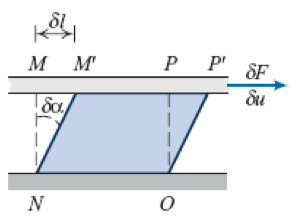
\includegraphics[width=.6\linewidth]{imgs/tens_cisa.png}
        \caption{Modelagem da Tensão de Cisalhamento}\label{img:tens_cis}
    \end{subfigure}% Really important to have this comment here and no black line
    \begin{subfigure}{.5\textwidth}
        \centering
        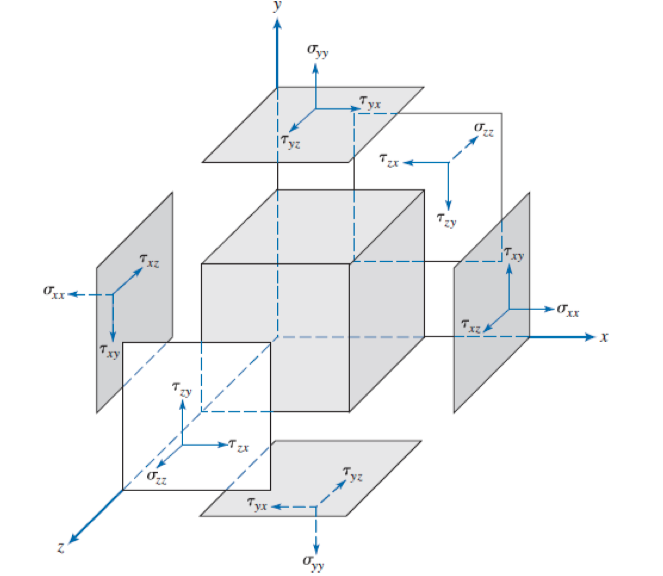
\includegraphics[width=.6\linewidth]{imgs/conv_tens.png}
        \caption{Convenção de Sinais de Tensão}\label{img:conv_sinais}
    \end{subfigure}
    \caption[]{Modelos para Tensão}
\end{figure}

A tensão de cisalhamento é uma tensão oriunda da movimentação relativa entre as faces externas de um fluido. Tal tensão é de suma importância pois, juntamente com a \textbf{condição de não
    escorregamento} (\emph{i.e} que o fluido, no ponto de contato com uma superfície, tem a mesma velocidade que tal superfície) nos possibilita calcular a força de resistência que o fluido
faz ao deslocamento.
Em primeiro lugar, a tensão de cisalhamento é dada por:
\begin{align}
    \tau_{yx} = \mu \frac{d}{dy} u, \begin{cases}
                                        \mu = Viscosidade \\
                                        u = Velocidade \ no \ eixo \ x
                                    \end{cases}
\end{align}

A partir disso, sabemos que força nada mais é que:
\begin{align}
    F_{reaction} = \tau_{yx} \cdot A, \ \ A= Contact \ Area
\end{align}


Algo importante de elaborarmos é a convenção de sinais para a tensão (e por conseguinte a força de reação). As tensões em um fluido seguem a convenção da imagem \ref{img:conv_sinais}. Isso
implica, se estamos observando a tensão da superfície superior do fluido, e ela é positiva, temos que ela aponta para a direita, já se estamos observando a tensão da superfície inferior
do fluido  e é positiva, temos que ela aponta para a esquerda.

\newpage
\subsection{One Pager - Conceitos Fundamentais}

\subsubsection*{Principais Fórmulas}

\begin{table}[h]\tiny
    \begin{tabularx}{\textwidth}{|l|c|X|}\hline
        \textbf{Nome}                          & \textbf{Equação}                                                                                              & \textbf{Descrição}                                                       \\ \hline

        \rule{0pt}{10ex} Linha de Corrente     & \begin{minipage}{0.5\textwidth}
                                                     $$\frac{dy}{dx} \big{)}_{linha \ de \ corrente} = \frac{v}{u}, \ \ \begin{cases}
                    v = v_y \\
                    u = v_x
                \end{cases}$$
                                                 \end{minipage} & Calculo da linha de corrente, que é tangente a velocidade em um ponto $x,y$. Podemos separar o que tem $x$ e $dx$ em um lado, $y$ e $dy$ do outro e integrar para achar
        uma função que depende de $xy$                                                                                                                                                                                                    \\[5ex] \hline

        \rule{0pt}{8ex} Tensão de Cisalhamento &
        \begin{minipage}{0.5 \textwidth}
            $$\tau_{yx} = \mu \frac{d}{dy} u, \begin{cases}
                    \mu = Viscosidade \\
                    u = Velocidade \ no \ eixo \ x
                \end{cases}$$
        \end{minipage}

                                               & Calculo da Tensão de cisalhamento, o resultado segue a convenção de sinais da imagem \ref{img:conv_sinais}.                                                                              \\[5ex] \hline

        \rule{0pt}{8ex} Força de Resistência   &
        \begin{minipage}{0.5 \textwidth}
            $$F_{reaction} = \tau_{yx} \cdot A, \ \ A= Contact \ Area$$
        \end{minipage}
                                               & Calculo da força de resistência ao movimento relativo entre duas placas com líquido no meio.                                                                                             \\[5ex] \hline
    \end{tabularx}

    $\\$
    $\\$

    \subsubsection*{Principais Conceitos}
    $\\$

        \begin{minipage}[c]{0.6 \textwidth}\tiny
            \begin{itemize}
                \item \textbf{Dimensões de Escoamento}:
                      \subitem $\hookrightarrow$ \underline{ Uni-Dimensional}: A velocidade muda em relação a somente uma coordenada.
                      \subitem $\hookrightarrow$ \underline{ Bi-Dimensional}: A velocidade muda em relação a  duas coordenadas.
                      \subitem $\hookrightarrow$ \underline{ Tri-Dimensional}: A velocidade muda em relação a três coordenadas.
                \item \textbf{Variação no Tempo}:
                      \subitem $\hookrightarrow$\underline{Regime Permanente}: A velocidade nem a massa específica variam com o tempo.
                      \subitem $\hookrightarrow$\underline{Regime Transiente}: As propriedades do fluido podem variar em relação ao tempo.
                \item \textbf{Princípio de Não Escorregamento}:O fluido, no ponto de contato com uma superfície, tem a mesma velocidade que tal superfície
            \end{itemize}
        \end{minipage}
        \begin{minipage}[c]{0.4 \textwidth}\tiny
            \begin{align*}
                \vec V = \vec V (x, y, z, t) = u \hat i + v \hat j + w \hat k
            \end{align*}
        \end{minipage}

    $\\$

    \subsubsection*{Convenções}\begin{figure}[H]
        \begin{subfigure}{0.5\textwidth}
            \centering
            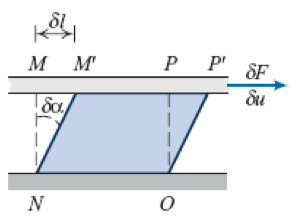
\includegraphics[width=.6\linewidth]{imgs/tens_cisa.png}
            \caption{Modelagem da Tensão de Cisalhamento}
        \end{subfigure}% Really important to have this comment here and no black line
        \begin{subfigure}{.5\textwidth}
            \centering
            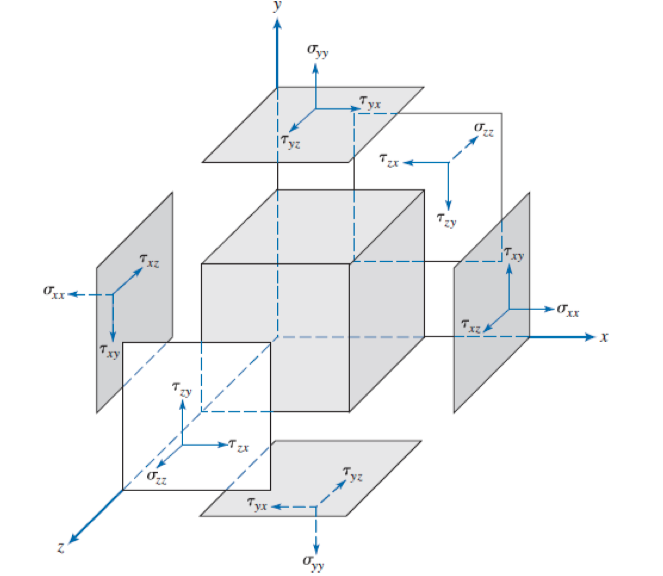
\includegraphics[width=.6\linewidth]{imgs/conv_tens.png}
            \caption{Convenção de Sinais de Tensão}
        \end{subfigure}
    \end{figure}



\end{table}
\newpage


\section{Equações Básicas na Forma Integral - Volume de Controle }
Agora vamos começar a ver mais detalhadamente as várias modelagens que podem nos auxiliar na análise de sistemas de Mecânica dos Fluidos.

\subsection{Modelagem Geral: Sistema $\rightarrow$ Volume de Controle}
De forma geral, a análise que mais somos familiares (desde a termo dinâmica com suas leis, etc) é a análise de Sistemas. Quando estamos lidando com fluidos, entretanto, modelarmos o problema como um
problema de análise de sistema se torna extremamente complexo, pois é muito difícil seguir a massa em todos os instantes (o que seria necessário já que um sistema não há troca de massa).
Por causa disso, iremos formular uma relação geral entre as relações que são verdade para um sistema (como leis da termodinâmica, conservação de quantidade de movimento, etc) e a aplicação em
um volume de controle.

Para uma propriedade extensiva\footnote{Extensiva no sentido de depender da quantidade de Matéria sob análise. Em contra partida Intensiva não depende da massa.} qualquer $N$ do sistema
temos que sua variação temporal, relacionada a variação no volume de controle é dada por:


\begin{align}
    \underbrace{\frac{dN}{dt}\big{)_{Sistema}}}_{Parte \ I} = \underbrace{\frac{\partial }{\partial t} \int_{VC} n \rho d \forall}_{Parte \ II} + \underbrace{\int_{SC} n \rho \vec V \cdot d \vec A}_{Parte \ III}
\end{align}

Onde:
\begin{itemize}
    \item Parte I - Representa a Taxa de variação da propriedade extensiva $N$ do sistema.
    \item Parte II - Representa a taxa de variação da propriedade $N$ dentro do volume de controle, com o termo $\int_{VC} n \rho d \forall$ representando o valor instantâneo de $N$.
    \item Parte III - Taxa na qual a propriedade $N$ está saindo pelas superfícies do volume de controle.
\end{itemize}

Podemos observar que para uma propriedade $N$ extensiva nós usamos para os calculos a propriedade intensiva $n$. Tal relação para cada propriedade de interesse para as nossas análises estão descritas na tabela abaixo:

\begin{table}[H]
    \begin{tabularx}{\textwidth}{|l|X|X|} \hline
        \textbf{Análise}                & \textbf{Propriedade Extensiva}                  & \textbf{Propriedade intensiva}                             \\ \hline
        Conservação de Massa            & $M \rightarrow$ Massa                           & $\rho \rightarrow$ Massa Específica                        \\ \hline
        Quantidade de Movimento Linear  & $H \rightarrow$ Quantidade de Movimento Linear  & $\vec V \rightarrow$  Velocidade                           \\ \hline
        Quantidade de Movimento Angular & $G \rightarrow$ Quantidade de Movimento Angular & $\vec r \times \vec V \rightarrow$  Braço vezes Velocidade \\ \hline
    \end{tabularx}
    \caption{Relação Geral entre Propriedade Extensiva e Propriedade Intensiva}
\end{table}

Agora veremos as diferentes análises que podemos fazer.

\subsection{Conservação de Massa}
Para a conservação de massa temos:
\begin{align}
    \frac{dM}{dt} = \frac{\partial}{\partial t} \int_{VC} \rho d\forall + \int_{SC}\rho \vec V \cdot d \vec A
\end{align}

Podemos, ainda, simplificar drasticamente para casos de \textbf{Regime Permanente}, \textbf{Perfil Linear de Velocidade} e \textbf{número constante de superfícies de controle}. Resultando em:
\begin{align}
    Q =  \sum V A = 0
\end{align}

Introduzimos ainda o conceito de \textbf{Vazão de Volume $Q$}, dado por $m^3/s$, que é \textbf{positivo} se o fluidos estiver saindo e \textbf{negativo} se estiver entrando.

\subsection{Conservação de Quantidade de Movimento Linear}
\subsubsection{Caso sem Velocidade Relativa}
Para a conservação de quantidade de movimento linear temos:
\begin{align}
    \frac{d \vec H}{dt} = \vec F = \vec F_S + \vec F_B = \frac{\partial}{\partial t} \int_{VC} \vec V \rho d\forall + \int_{SC}\vec V \rho \vec V \cdot d \vec A
\end{align}

Que pode ser decomposto para as 3 componentes da velocidade $V$, resultando em 3 equações que não são vetoriais (o que facilita bastante):
\begin{align}
    F_x = \vec F_{S_x} + \vec F_{B_x} = \frac{\partial}{\partial t} \int_{VC} \vec u \rho d\forall + \int_{SC}\vec u \rho \vec V \cdot d \vec A \n
    F_y = \vec F_{S_y} + \vec F_{B_y} = \frac{\partial}{\partial t} \int_{VC} \vec v \rho d\forall + \int_{SC}\vec v \rho \vec V \cdot d \vec A \n
    F_z = \vec F_{S_z} + \vec F_{B_z} = \frac{\partial}{\partial t} \int_{VC} \vec w \rho d\forall + \int_{SC}\vec w \rho \vec V \cdot d \vec A
    \label{eq:cons_quan_movi_lin}
\end{align}

Onde as \textbf{forças representadas são as forças externas ao volume de controle para manter o cenário cinemático} (de velocidade constante nula ), como por exemplo $F_{s_x} = F_{at}$.

Importante, também, ressaltar que cada superfície de controle do nosso volume de controle terá um $\vec V$ e um $\{u, v, w\}$ específico, e que é bom usar um subscrito para identificar (\emph{e.g} $u_1$ e $u_2$).

Além disso, é de suma importância perceber que as velocidades de entrada \textbf{{u, v, w} possuem um sinal (a depender dos eixos das coordenadas)} e que a expressão \textbf{$\vec V dA$ também possui sinal, sendo ele positivo se o fluido estiver saindo e negativo se estiver entrando}.

\subsubsection{Caso com Velocidade Relativa Constante}
Para o caso em que a volume de controle possui velocidade constante, ocorre a situação em que há uma velocidade relativa entre o jato de água e a superfície de controle, que precisa ser levada em consideração.

Para exemplificar a situação acima, vamos imaginar que um bocal esteja lançando um jato de água com uma velocidade no eixo $x$ de $V_j = V \hat i$. Além disso, um cano em formato de $\supset$ está andando a uma velocidade \textbf{Constante} $U$ (também no eixo $x$). Como estamos lidando
com velocidades constantes não há acelerações e, para tal, há a presença de uma força de resistência $R_x$ que impede a aceleração que seria oriunda da força necessária para virar o jato de água.

Ao analisarmos o volume de controle, há duas superfícies de controle, $1$ e $2$. Que possuem, por conservação de massa, as mesma velocidades de fluido entrando, sendo esse $|V_1| = |V_2| = V - U$. A partir disso somos capazes de aplicar a equação  \ref{eq:cons_quan_movi_lin} para o eixo $x$. Dando ênfase nos sinais tanto das velocidades {u, v, w} de entrada das superfícies de controle quanto no sinal oriundo do fato de estar entrando ou saindo do VC, dado pela parcela $VA$ ou $VdA$.

\subsubsection{Caso com Aceleração Constante}
Já para o caso onde há aceleração constante, temos que parte da quantidade de movimento é utilizada para acelerar o anteparo, e outra para "vencer" as forças externas de reação $F_{S}$ e $F_{B}$, resultando na seguinte equação:

\begin{align}
    \vec{F}_{S} + \vec{F}_B - \int_{VC} \vec{a} \rho d\forall = \frac{\partial}{\partial t}\int_{VC}\vec V \rho d\forall + \int_{SC} \vec V \rho \vec V\cdot d \vec A
\end{align}

E, que de forma análoga a como foi feito para o caso sem aceleração, pode ser expandido para suas $3$ componentes.

\newpage
\subsection{Conservação de Energia}
A partir da conservação de energia, e da segunda lei da termo-dinâmica, obtemos a seguinte equação:

\begin{align}
    \dot Q - \dot W_s - \dot{W}_{cisalhamento} - \dot{W}_{others} = \frac{\partial}{\partial t}\int_{VC} e \rho d\forall + \int_{SC} \left(u + \rho^{-1} p + \frac{V^2}{2} + gz\right) \rho \vec V \cdot d\vec A
\end{align}

Onde $e$ representa a Energia Específica do fluido.

Além disso, podemos também descrever tal equação exaltando a entalpia $h$:

\begin{minipage}{.5\textwidth}
    \begin{align*}
        h = u + P \rho^{-1}
    \end{align*}
\end{minipage}
\begin{minipage}{.5\textwidth}
    \begin{align*}
        \Delta h = c_p \Delta T
    \end{align*}
\end{minipage}

\subsection{Equação de Bernoulli}
Outra equação que é muito útil é a \emph{Equação de Bernoulli}, que nos possibilita calcular certos parâmetros nos casos onde há uma diferênça considerável de altura, pressão, etc. Sendo válida somente para os casos de:
\begin{itemize}
    \item Escoamento Permanente
    \item Ausência de Atrito
    \item Escoamento ao longo de uma linha de corrente (normalmente sempre é para nossos exercícios)
    \item Escoamento incompressível
    \item Isotérmico
\end{itemize}

\begin{align}
    \frac{P_1}{\rho_1} + \frac{V^2_1}{2} + gz_1 = \frac{P_2}{\rho_2} + \frac{V^2_2}{2} + gz_2
\end{align}

\newpage
\section{Análise Dimensional e Semelhança}
\subsection{Análise Dimensional - Introdução}


Como podemos ver com os tópicos vistos até agora, a mecânica de fluidos é uma matéria que para seu entendimento e sua modelagem são necessários inúmeros parâmetros diferentes, desde aqueles referentes
ao fluido (como $\rho$ e $\mu$) até aqueles referentes aos objetos sendo afetados pelo fluxo e geometria das tubulações, etc.

Além disso, temos que por ser uma área tão complexa muitas das vezes a derivação dos modelos matemáticos puramente pela teoria e analiticamente são inviáveis, resultando na necessidade recorrente de se fazer experimentos
em laboratórios tanto para pequenos modelos quanto para grandes protótipos.

Esses dois fatores juntos resultam em uma combinação extremamente cara, pois experimentos são necessários de serem refeitos para cada pequena alteração dos inúmeros parâmetros envolvidos, a fim de tentar entender a contribuição de cada um para o sistema como um todo.

\begin{wrapfigure}{r}{.5\textwidth}
    \centering
    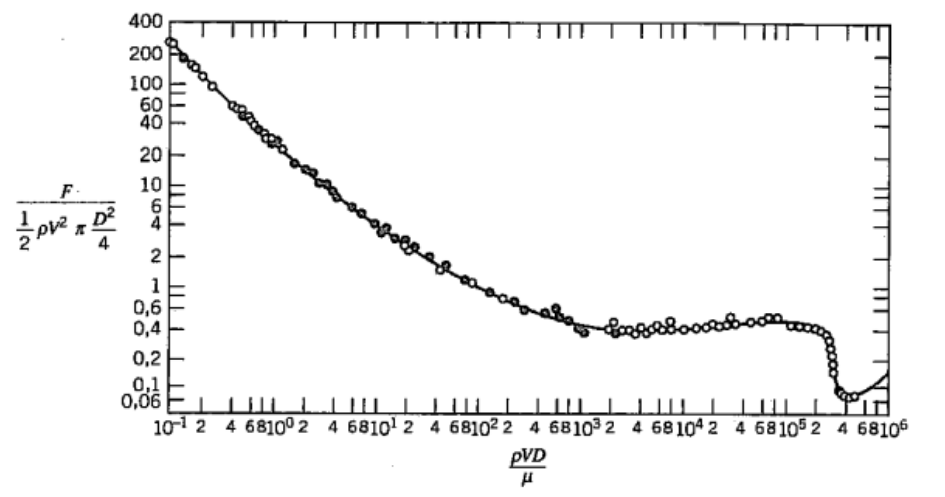
\includegraphics[width=.5\textwidth]{imgs/adm_analysis.png}
\end{wrapfigure}

A fim de facilitar entender a relação dos vários parâmetros com o sistema, são desenvolvidos \textbf{Números/ Parâmetros Adimensionais}, a fim de agrupar a maior quantidade desses fatores juntos de uma forma
a se obter fatores sem dimensão de unidade, facilitando a modelagem dos sistemas. Um exemplo disso é a junção, no caso de uma esfera submetida a escoamento de ar, das influências do diâmetro e rugosidade da bola, velocidade que viaja e seu spin em um único fator adimensional, para que possamos então vermos a relação da força de arrasto em função de somente uma variável, ao invés de várias, fazendo com que
o curve-fitting para achar o modelo seja de uma dimensão só (como \emph{ilustrado} pela figura ao lado).

O método utilizado para acharmos tais fatores adimensionais é chamado de \textbf{Teorema de $\Pi$ Buckingham}.

\subsection{Teorema de $\Pi$ Buckingham}

A partir de um problema físico, onde queremos modelar uma variável $q_1$ \textbf{dependente} de outras $n-1$ variáveis \emph{independentes} $\{q_2, q_3, q_4, ..., q_{n}\}$ assumindo a forma $q_1 = f(q_2, q_2, ..., q_n)$ somos capazes modelar a relação de todas as variáveis também em forma funcional como sendo $g(q_1, q_2, ..., q_n) = 0$ onde $f$ e $g$ são funções distintas.

É a partir dessa capacidade de relacionar \textbf{todas} as variáveis em uma função que o teorema de $\Pi$ se pauta para dizer que:

\begin{center}
    \textbf{Dada uma relação entre $n$ parâmetros na forma $g(...)=0$ os $n$ parâmetros podem ser agrupados em $n-m$ parâmetros/razões adimensionais independentes, chamadas de parâmetros $\Pi$}
\end{center}

Onde $m$ representa\footnote{Isso nem sempre é verdade, mas para os nossos estudos iremos assumir que $m=r$ sempre.} o número $r$ de dimensões independentes mínimas para expressar todas as dimensões/unidades das variáveis $\{q_1, ..., q_n\}$.

Para achar os $\Pi$ valores temos que seguir os seguintes passos:
\begin{enumerate}
    \item Liste todas as $n$ unidades das $n$ variáveis (tanto a independente quanto as dependentes).
    \item Selecione um conjunto de dimensões fundamentais (o mais comum sendo $M$: Massa, $L$: Distância e $t$: Tempo).
    \item Liste todas as $n$ unidades em função das unidades fundamentais ($MLt$)
    \item Selecione, a partir das lista de $n$ unidades das variáveis, um conjunto que inclua todas as dimensões primárias. Essa lista será chamada de \emph{parâmetros repetentes} e normalmente são escolhidos $(\rho, V, D)$, ou então uma do fluido, uma de velocidade do corpo e uma da geometria do corpo.
    \item Forme as equações dimensionais, combinando os parâmetros repetentes escolhidos acima, cada um elevado a uma potência, com as outras unidades restante, uma equação para cada parâmetro restante.
    \item Ache as potências supracitadas para que cada equação seja adimensional.
\end{enumerate}

\subsection{Modelos e Semelhança}
Como dito anteriormente, grande parte de mecânica dos fluidos é oriunda de experimentos laboratoriais. Muitas das vezes, entretanto, estamos lidando com grandes construção (\emph{e.g} navius, aviões, etc) e isso significa que ter que construir toda a estrutura para saber como que ela irá se comportar
não é viável. Para tal, precisamos criar modelos em escala para que possamos testa-los e somente depois construir os protótipos em si.

Para que tais modelos gerem resultados cabiveis de serem usados, é necessário garantir a sua \textbf{semelhança} com sua contraparte de escala maior. Para tal é encessário garantir:
\begin{itemize}
    \item \textbf{Semelhança Geométrica}: As relações entre as dimensões do modelo e do protótipo precisam ser mantidas.
    \item \textbf{Semelhança Cinemática}: Velocidades em pontos correspondentes precisam ter mesma direção e sentido, diferindo apenas pelo módulo, por um fator de escala constante.
    \item \textbf{Semelhança Dinâmica}: A distribuição de forças precisa ter mesma direção e sentido, diferindo apenas pelo módulo, por um fator de escala constante.
\end{itemize}

Isso implica, também, que os números adimensionais do modelo são iguais ao do protótipo.

\newpage
\section{Escoamento Interno e Viscoso}
Até o momento, sempre desprezamos os efeito da viscosidade e, por conseguinte, quaisquer perdas de energia devido a ela. A partir de agora, entretanto, iremos estudar a forma de modelar tais perdas, tanto para fluxos laminares quanto turbulentos.

\subsection{Perdas de Carga - Formulação Geral}
A perda de carga, de forma geral dada devido à viscosidade do fluido, pode ser dividida em dois tipos:
\begin{itemize}
    \item Perdas Localizadas: Em decorrência da mudança (a partir de certo ponto) da área da tubulação, da presença de válvula, entre outras coisas.
    \item Perdas Distribuídas: Em decorrência de atritos em trechos de área constante.
\end{itemize}

Mas, independente de tais perdas, a seguinte lei de conservação de energia é aplicável (e usaremos muito ela para a solução de problemas com perda de carga):
\begin{align}
    \left(\frac{p_1}{\rho} + \alpha_1 \frac{\bar{V}^2_1}{2} + gz_1\right) - \left(\frac{p_2}{\rho} + \alpha_2 \frac{\bar{V}^2_2}{2} + gz_2\right) = h_{l_{T}} = h_{l_{Local}} + h_{l_{Dis}}
\end{align}

Onde:
\begin{itemize}
    \item $\alpha$: Representa um coeficiente de energia cinética, que para problemas de escoamento laminar $\alpha_{lam} = 2$ e para problemas de escoamento turbulento (e sempre aplicável para escoamento em tubos) $\alpha_{turb} = 1$
    \item $h_{l_{T}}$: Representa a perda total de carga.
    \item $h_{l_{Local}}$: Representa a soma de todas as perda de carga localizadas.
    \item $h_{l_{Dis}}$: Representa a soma de todas as Distribuídas de carga.
\end{itemize}

\newpage
\subsection{Perdas Distribuídas}

De forma geral, temos que a perda de carga distribuída é dada pela seguinte equação:
\begin{align}
    h_{l} = f \frac{L}{D}\frac{\bar{V}^2}{2}
    \label{eq:perda_carga_distribuida}
\end{align}

Onde podemos ver que a carga perdida $h_l$ é em função de $f$, que é chamado de \textbf{Fator de Atrito}, sendo esse dependente tanto do tipo de fluxo (laminar ou turbulento) mas também do tipo de tubo no qual o escoamento ocorre, sua rugosidade, ferrugem, etc.

Para acharmos tal fator de atrito, podemos utilizar tanto o diagrama de Moody (imagem \ref{img:moody_chart}) ou ainda por algumas equações (mostradas na tabela \ref{tab:fator_atrito}), onde cada uma é aplicável para um cenário específico (\emph{i.e} um Reynalds Específico).

\begin{figure}[h]
    \centering
    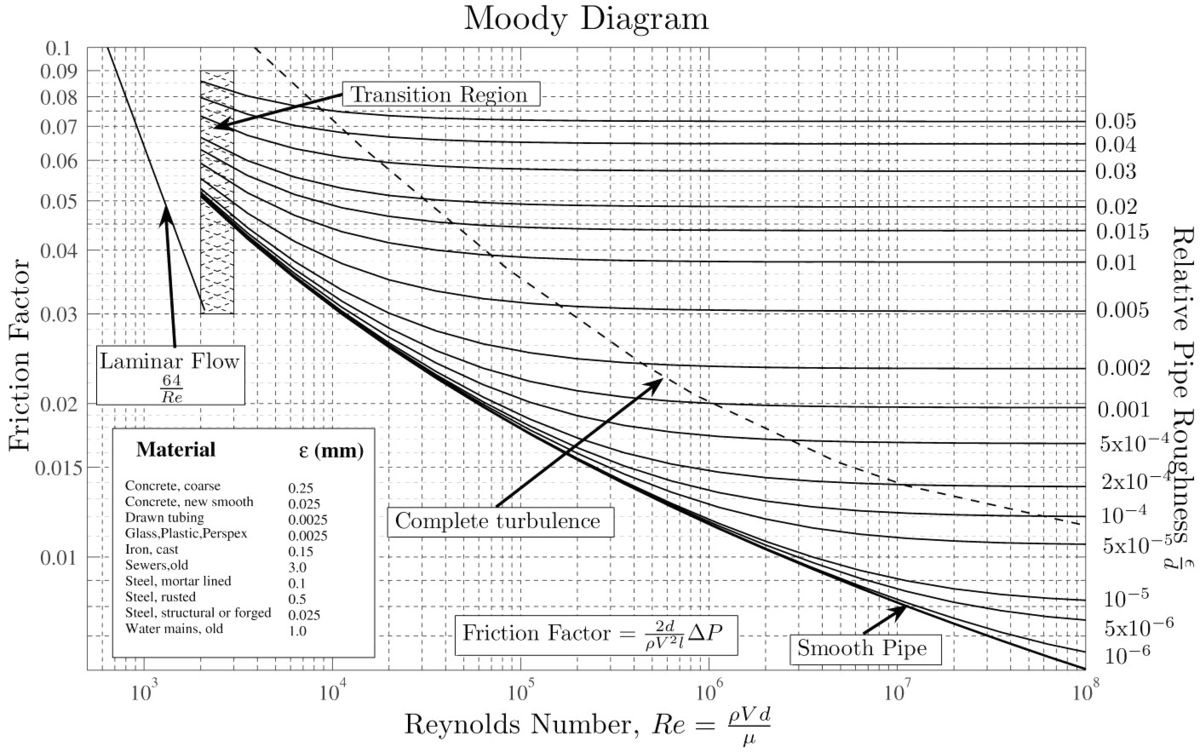
\includegraphics[width=\textwidth]{imgs/moody_chart.jpg}
    \caption{Diagrama de Moody - Fator de Atrito parametrizado}
    \label{img:moody_chart}
\end{figure}


\begin{table}[h]
    \begin{tabularx}{\textwidth}{|X|X|X|}\hline
        \textbf{Nome}           & \textbf{Equação}                                                               & \textbf{Descrição e Uso}                                                                                                                         \\ \hline
        Fator de Atrito Laminar & $f_{laminar} = 64/Re$                                                          & Fator de Atrito a ser usado quando o escoamento se enquadra em laminar.                                                                          \\ \hline
        Fórmula de Colenbrook   & $f^{-0.5} = -2 \log\left(\frac{eD^{-1}}{3.7} + \frac{2.51}{Re f^{0.5}}\right)$ & Usado para escoamentos turbulentos, e é preciso resolver de forma iterativa, tendo em vista que a variável $f$ está em ambos os lados da equação \\ \hline
        Fórmula de Blausius     & $f = 0.316/(Re^{0.25})$                                                        & Usando para Escoamentos Turbulentos, com $Re<10^5$                                                                                               \\ \hline
    \end{tabularx}
    \caption{Tabela de Fórmulas do Fator de Atrito}
    \label{tab:fator_atrito}
\end{table}

\subsection{Perdas Localizadas}
Podemos representar o calculo de perdas localizadas das duas formas abaixo:

\begin{minipage}{.4\textwidth}
    \begin{align}
        h_{l_m} = K \frac{\bar{V}^2}{2}
        \label{eq:perda_carga_local_forma_1}
    \end{align}
\end{minipage}
\begin{minipage}{.5\textwidth}
    \begin{align}
        h_{l_m} = f \frac{L_e}{D} \frac{\bar{V}^2}{2}
        \label{eq:perda_carga_local_forma_2}
    \end{align}
\end{minipage}

$$ $$

A equação mais utiliza é a forma da equação \ref{eq:perda_carga_local_forma_1}, onde $K$ representa uma constante dependente do tipo de restrição do fluxo que resulta na perda de carga.

Podemos, entretanto, usar a forma da equação \ref{eq:perda_carga_local_forma_2} pois faz uma referência à formulação da carga distribuída (eq. \ref{eq:perda_carga_distribuida}), possibilitando fazer um paralelo de "Quantos Metros A mais de Perda Distribuída essa perda localizada equivale", tendo em
vista que ambas as formulações distribuídas e localizadas ficam em função um comprimento, sendo no caso da formulação distribuída a distância real e no caso da formulação localizada uma distância "Equivalente".

Ocorrerá a perda localizada sempre que no sistema sob análise houver:
\begin{itemize}
    \item Entradas e Saídas
    \item Expansões e Contrações
    \item Curvas em tubos
    \item Válvulas e Acessórios
\end{itemize}

\subsection{Ganho de Cargas}
Até o momento vimos as diferentes topologias e suas modelagens que geram a \emph{perda} de carga para um fluido submetido a escoamento viscoso interno. Há, entretanto,
também o cenário onde carga é injetada em um fluido, através de \textbf{bombas, ventiladores e sopradores}.

Para tais casos, temos a seguinte formulação:
\begin{align}
    \left(\frac{p_1}{\rho} + \alpha_1 \frac{\bar{V}^2_1}{2} + gz_1\right) - \left(\frac{p_2}{\rho} + \alpha_2 \frac{\bar{V}^2_2}{2} + gz_2\right) = h_{l_{T}} = h_{l_{total}} - \Delta h_{bomba}
\end{align}

Onde vale re-lembrar que, pela segunda lei da termo dinâmica, podemos encontrar a potência da bomba $\dot W$ em função da vazão volumétrica $Q$ e diferencial de pressão $\Delta P$ (ou vice-versa):
\begin{align}
    \dot W_{Bomba} = Q\Delta P
\end{align}

\newpage
\section{Escoamento Externo e Viscoso}
\subsection{Introdução}

Quando ocorre o escoamento de fluido ao redor de um corpo, chamamos de escoamento externo. Nesses casos, na maior parte das vezes o que mais nos interessa é saber as forças sofridas pelo corpo devido à esse movimento
relativo (como por exemplo a força de lift e a força de drag sofrida por uma asa de avião).

Tais forças são originadas a partir das forças de pressão e forças de cisalhamento. A distinção entre a componente de uma e outra, entretanto, é extremamente difícil (se não impossível) a depender do fluxo e da geometria.
Levando isso em consideração, juntamente com os objetivos das modelagens de escoamentos externos, nós dividimos as forças não devido a suas origens, mas sim devido a sua \emph{direção relativa ao escoamento}, obtendo então:
\begin{itemize}
    \item \textbf{Força de Drag $F_D$}: uma força na direção do escoamento, parametrizada por $C_D$.
    \item \textbf{Força de Lift $F_L$}: uma força perpendicular ao escoamento, parametrizada por $C_L$.
\end{itemize}

\subsection{Força de Drag}
Como dito anteriormente, a força de drag é a força gera perpendicularmente ao escoamento do fluido em relação a um corpo. Por ser um problema que envolve muitas variáveis
(como geometria do objeto, velocidade, viscosidade do fluido, etc) a análise da força de arrasto (força de drag) é muito mais fácil de ser feita aplicando análise dimensional e achando um parâmetro adimensional (utilizando o teorema de Pi Buckingham).

Parametrizando então a força de drag foi desenvolvida o coeficiente de arrasto (ou coeficiente de drag) $C_D$:
\begin{align}
    C_D = \frac{F_D}{\frac{1}{2}\rho V^2 A} = f(Re)
\end{align}

Existem diferentes valores para $C_D$, a depender principalmente do tipo de fluxo (se é laminar ou turbulento) e da geometria, que são tabulados.

A partir desses valores conhecidos de $C_D$, somos capazes de aplicar a equação acima e isolarmos a força:
\begin{align}
    F_D = C_D \left(\frac{1}{2} \rho V^2 A\right)
\end{align}

\subsection{Força de Lift}

De forma análoga a como a força de drag é parametrizada por um parâmetro adimensional a fim de facilitar seu estudo, a força de Lift (também chamada de força de sustentação), que é a parcela da força perpendicular ao movimento do fluido em relação ao corpo,
também é parametrizado pelo chamado \textbf{Coeficiente de Sustentaçõa}, dado por:
\begin{align}
    C_L = \frac{F_L}{\frac{1}{2}\rho V^2 A} = f(Re)
\end{align}

Onde podemos, também, isolar a força e deixa-la em função do coeficiente:
\begin{align}
    F_L = C_L \left(\frac{1}{2} \rho V^2 A\right)
\end{align}

\end{document}